%%% Document class beamer, do not change
\documentclass[t,professionalfont,10pt]{beamer}
%\documentclass[article]{beamer}
%\usepackage{pgfpages}
%\setbeameroption{show notes} 
%\setbeameroption{show notes on second screen=right} 
%\setbeameroption{show only notes} 
\usepackage{listings}
\usepackage{subcaption}
\usepackage{booktabs,topcapt,rccol,tabularx,multirow,siunitx}
\newcommand{\otoprule}{\midrule[\heavyrulewidth]}

% FONTS & LANGUAGE
\usepackage{fontspec}
\usepackage{xltxtra}
\usepackage[normalem]{ulem} % have underlinings work
\usepackage{unicode-math}

% \DeclareMathSizes{9.8}{17}{7}{7}
% \DeclareMathSizes{10}{17}{7}{7}
% \DeclareMathSizes{10.95}{12}{8}{8}   % For size 10 text
% \DeclareMathSizes{11}{19}{13}{9}      % For size 11 text
% \DeclareMathSizes{12}{20}{14}{10}     % For size 12 text

% MATH
\usepackage{mymath}

\usepackage{amsthm}
\usepackage{enumerate}
\usepackage{xfrac}
%\DeclareMathSizes{12}{15}{13}{12}
\newcommand{\matlab}{\textsc{Matlab}}
\newcommand{\yk}{\v{y}_{k}}
\newcommand{\y}{\v{y}}
\newcommand{\ykk}{\v{y}_{k-1}}
\newcommand{\xk}{\v{x}_{k}}
\newcommand{\x}{\v{x}}
\newcommand{\X}{\x_{0:T}}
\newcommand{\XX}{\v{X}}
\newcommand{\Y}{\y_{0:T}}
\newcommand{\YY}{\v{Y}}
\newcommand{\z}{\v{z}}
\newcommand{\h}{\v{h}}
\newcommand{\f}{\v{f}}
\newcommand{\g}{\v{g}}
\newcommand{\p}{\v{p}}
\newcommand{\q}{\v{q}}
\newcommand{\ym}{\v{\mu}_k}
\renewcommand{\S}{\v{S}_k}
\NewDocumentCommand\sig{G{j}}{\v{\varsigma}^{(#1)}}
\NewDocumentCommand\usig{G{j}}{\v{\varepsilon}^{(#1)}}
\NewDocumentCommand\jacob{O{\big} m m}{\F[#1]{\v{J}_{#2}}{#3}}

\renewcommand{\P}{\v{P}}
\renewcommand{\m}{\v{m}}
\newcommand{\xkk}{\v{x}_{k-1}}
\newcommand{\tr}{\mathsf{T}}
\newcommand{\Th}{\v{\theta}}

\newcommand{\rTh}{\textcolor{cyan}{\theta}}

\NewDocumentCommand\lLH{O{\Th}}{\F[\big]{\ell}{#1}}
\NewDocumentCommand\score{}{\nabla\lLH}
\NewDocumentCommand\Hess{}{\nabla^2\lLH}
\NewDocumentCommand\ene{G{\Th}}{\F[\big]{\varphi}{#1}}
%\newcommand{\LHf}[1]{\Pdf{\X}{#1}}
%\newcommand{\LHh}{\Pdf{\X}{\hat{\Th}}}
%\newcommand{\lLH}{\ell\!\left(\Th\right)}
%\newcommand{\cLH}{\Pdf{\X,\Y}{\Th}}
%\newcommand{\lcLH}{\log\cLH}
\newcommand{\tP}{q}
\NewDocumentCommand\tPX{O{\tP} G{\v{\psi}}}{\Pdf[#1]{\X}{#2}}
\NewDocumentCommand\ff{O{\displaysize} G{\xkk} G{\Th}}{\F[#1]{\f}{#2,#3}}
\NewDocumentCommand\hh{O{\displaysize} G{\xk} G{\Th}}{\F[#1]{\h}{#2,#3}}
\NewDocumentCommand\ffi{O{\displaysize} G{\xkk}}{\F[#1]{\f}{#2}}
\NewDocumentCommand\hhi{O{\displaysize} G{\xk}}{\F[#1]{\h}{#2}}
\NewDocumentCommand\QQ{s G{\Th}}{\IfBooleanTF{#1}{\v{Q}}{\F{\v{Q}}{#2}}}
\NewDocumentCommand\RR{s G{\Th}}{\IfBooleanTF{#1}{\v{R}}{\F{\v{R}}{#2}}}
\NewDocumentCommand\muu{s G{\Th}}{\IfBooleanTF{#1}{\v\mu_0}{\F{\v\mu_0}{#2}}}
\NewDocumentCommand\Sig{s G{\Th}}{\IfBooleanTF{#1}{\v\Sigma_0}{\F{\v\Sigma_0}{#2}}}
\NewDocumentCommand\II{O{\displaysize} m}{\F[#1]{\v{I}_{#2}}{\Th,\Th'}}
\NewDocumentCommand\III{O{\displaysize} m}{\F[#1]{\widehat{\v{I}}_{#2}}{\Th,\Th'}}
\NewDocumentCommand\post{G{\Th}}{\Pdf[p]{\X}{\Y,#1}}
\NewDocumentCommand\cLH{G{\Th}}{\Pdf{\X,\Y}{#1}}
\NewDocumentCommand\LH{G{\Th}}{\Pdf{\Y}{#1}}
%\NewDocumentCommand\lcLH{O{0pt}}{\log\cLH[#1]}
\NewDocumentCommand\EMQ{o G{\Th'} G{\Th}}{
	\IfNoValueTF{#1}
		{\F{\mathcal Q}{#3,#2}}
		{\F[#1]{\mathcal Q}{#3,#2}}
}
\NewDocumentCommand\EMH{G{\Th'} G{\Th}}{\F{\mathcal H}{#2,#1}}
\NewDocumentCommand\EMB{G{\Th'} G{\Th}}{\F[\big]{\mathcal B}{#2,#1}}
\NewDocumentCommand\EMM{s O{} G{\Th}}{
	\IfBooleanTF{#1}
		{\v{M}}
		{\F{\v{M}#2}{#3}}
}
\newcommand{\KL}[2]{\mathrm{KL}\fparenmid[\big]{#1}{#2}{\Vert}}

\NewDocumentCommand\dQ{O{2} O{0} G{\Th_\star} G{\Th_\star}}{
	\nabla^#1\EMQ{#4}{#3}
}
\NewDocumentCommand\dH{O{2} O{0} G{\Th_\star} G{\Th_\star}}{
	\nabla^#1\EMH{#4}{#3}
}
\NewDocumentCommand\dL{O{2} O{0} G{\Th_\star}}{
	\nabla^#1\lLH[#3]
}
\NewDocumentCommand\prtdd{m G{\Th} g}{
	\IfNoValueTF{#3}
		{\dpd[2]{#1}{#2}}
		{\dmd{#1}{2}{#2}{}{\left.\mkern-2mu #3^\tr \right.}{}}
}

\usepackage{tikz}
\usetikzlibrary{arrows,backgrounds}

%% Input the document information, note the use of short information in the footer
% The document title. Shows an example how linebreaks can be obtained.
\title[Gauss. filtering and smoothing based param. est. \ldots]{%
Gaussian filtering and smoothing based parameter estimation in nonlinear models for sequential data
}

% The subtitle, e.g. the conference or course name.
% An abbreviation (or similar) in the short version is handy.
\subtitle[Master's thesis presentation]{%
Master's thesis presentation
}



% The author names. Shows a second example of linebreaks.
% Note the use of \inst, see the \institute command!
\author[Väänänen]{%
	Ville Väänänen\\
	{\scriptsize\url{ville.vaananen@aalto.fi}}
}
% The authors' affiliations.
\institute[Aalto ELEC]{%
%	Department of Biomedical Engineering and Computational Science\\
	Aalto University School of Electrical Engineering
}
% The date. Default date is \today.
%\date[Short Example Date]{%
%	Long Example Date, Default Date is \textbackslash today%
%}
% The subject. This is stored only in the PDF information.
\subject{Document Subject Example}

%\usepackage{mylayout}

% Theme loading
\usepackage[ELEC]{aaltologo}
\usetheme{Aalto}
%\setmathfont{xits-math.otf}
\setmathfont{Asana-Math.otf}
%\setmathfont{lmmath-regular.otf}

%\usefontheme{professionalfont}

% \setmainfont
%   [  
%   	Path=/usr/local/texlive/2012/texmf-dist/fonts/opentype/public/xits/,
%     Extension=.otf,
%    UprightFont = *-regular,
%       BoldFont = *-bold,
%     ItalicFont = *-italic,
% BoldItalicFont = *-bolditalic,
% ]{xits}




%%% Begin the document
\begin{document}
\makeatletter
 \def\beamer@framenotesbegin{% at beginning of slide
   \gdef\beamer@noteitems{}%
   \gdef\beamer@notes{{}}% used to be totally empty.
 }
 \makeatother
%%% This file contains the code for the sample0x.tex files.

%% Create the title page
\maketitle

\begin{frame}
	\frametitle{Outline}
	\tableofcontents
	\note{blaa}
	% You might wish to add the option [pausesections]
\end{frame}


\section{Introductory application}
\begin{frame}[fragile]
	\frametitle{Ballistic object on reentry, dynamics}
	 %\tikz[baseline,overlay]\node{
		%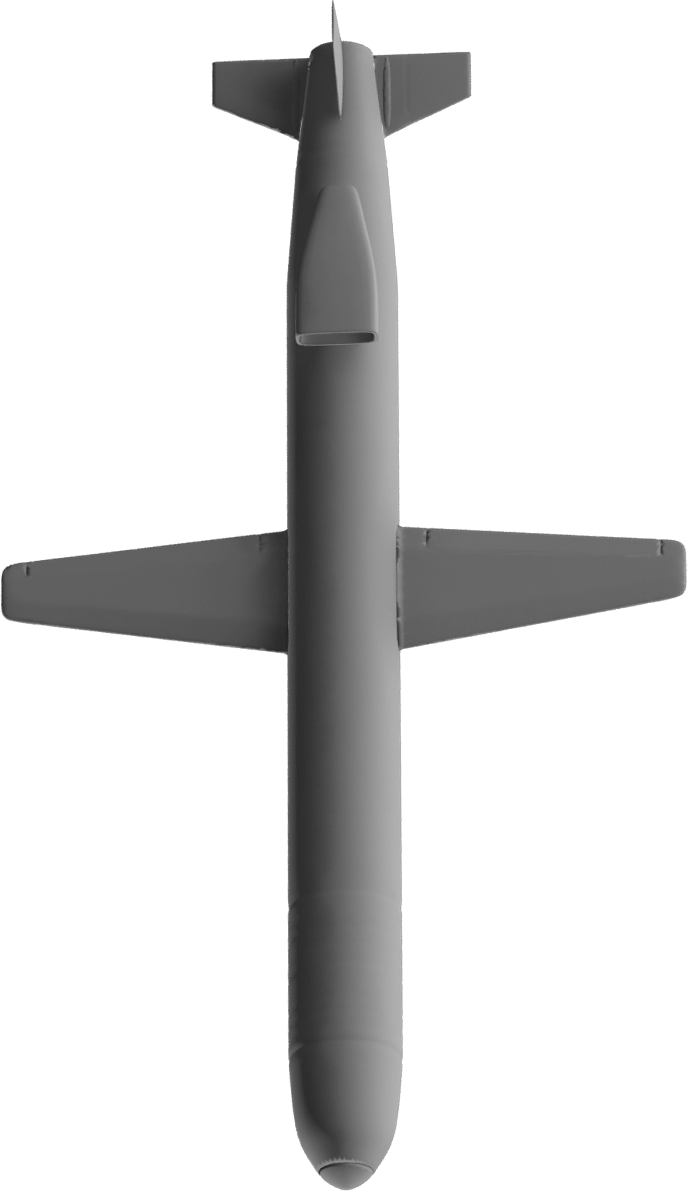
\includegraphics[width=\textwidth]{fig/missile}
	%	dfgdf dfgd 
	%}
	\note[itemize]{
	\item boost phase (thrust acceleration), ballistic phase, reentry phase
	\item the missile moves in one dimension, Newtons mechanics
	\item drag force: proportional to ballistic coefficient, air density and the velocity squared
	\item SDE: beta can be thought of as a white noise process
	 } 
	\begin{itemize}\large
	  %\item<2>$\rho(h)=e^{-\eta\,h}$
	  \item<2>$d(h,v,\rTh) = \rTh\,\rho(h)\,v^2$
	  \item<2> $\dod{}{t}\bm{h(t)\\v(t)} = 
	  \bm{-v(t) \\ g-d\fparen[\big]{h(t),v(t),\rTh}}+\bm{0\\1}w(t)$
	  \item<3> $\xk = \bm{h_k & v_k}^\tr$
	  \item<3> $\xkk = \bm{1&-\tau\\&1}\xk+%
	  \bm{0 \\ \tau}\fparen[\Big]{g-d\fparen[\big]{x_{k,1},x_{k,2},\rTh}}+\v{q}_{k-1}$
	  \item<3> $\v{q}_{k-1} \sim \N{\v{0}}{\v{Q}}$ 
	\end{itemize}
	\hfill%
	\begin{tikzpicture}[remember picture, overlay]
    	\tikzstyle{cog}=[circle, minimum size = 1.5mm, inner sep=0mm, node distance = 0mm,fill=white,draw=red]
    	\tikzstyle{connect}=[-latex, thick, fill=white, draw=red]
    	\node[inner sep=0pt] at (-0.9cm,3.5cm) {%
        	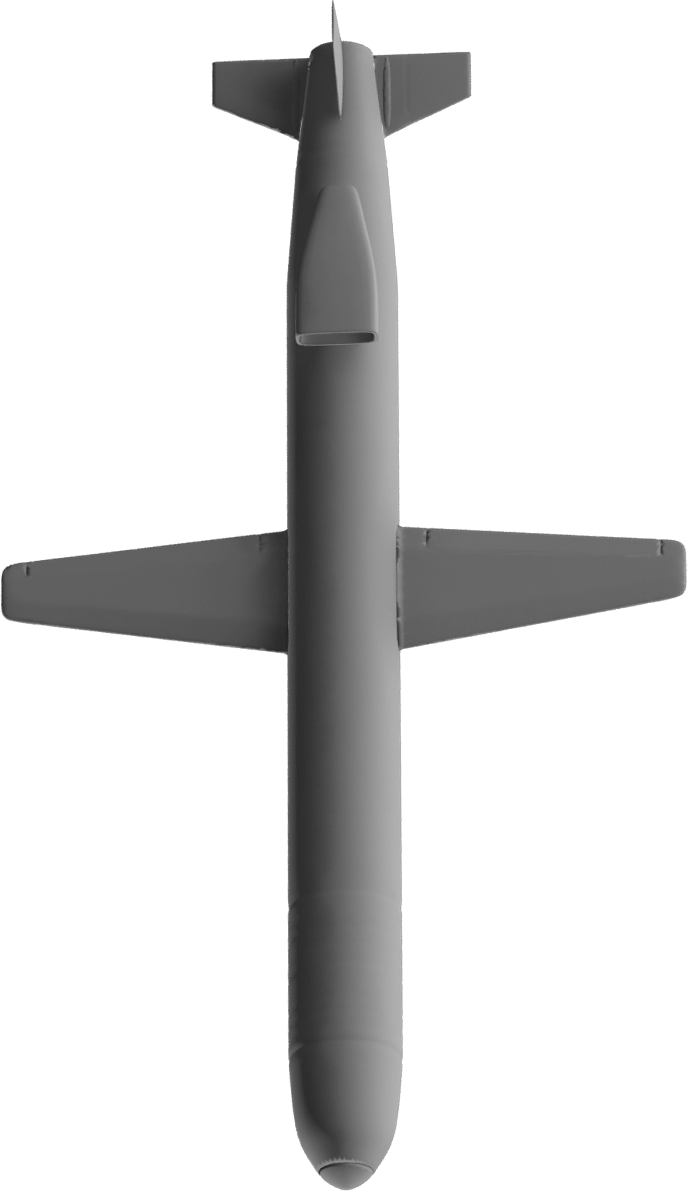
\includegraphics[height=0.65\paperheight]{fig/missile}%
    	};%
    	\node[cog] (x) at (-0.9cm,3.6cm){};
    	\node (d) [above of = x,node distance=1.4cm,label={[label distance=0.15cm]-20:{\color{red}$d(h,v,\rTh)$}}]{};
    	\node (g) [below of = x,node distance=2.4cm,label={[label distance=0.15cm,text=red]20:$g$}]{};
    	\path
	    (x) edge [connect] (g)
	    	edge [connect] (d);
	\end{tikzpicture}

\end{frame}

\begin{frame}
	\frametitle{Ballistic object on reentry, measurements}
	%\vskip -15pt
	\note{long range radar, anti-ballistic missile}
	\begin{itemize}\large
	  \item $\yk = \bm{0 & 1}\xk + r_k $
	  \item $r_k \sim \N{0}{\sigma_r^2}$ 
	\end{itemize}
	\hfill%
	\begin{tikzpicture}[remember picture, overlay]
    	\tikzstyle{cog}=[circle, minimum size = 1.5mm, inner sep=0mm, node distance = 0mm,fill=white,draw=red]
    	\tikzstyle{connect}=[-latex, thick, fill=white, draw=red]
    	\node[inner sep=0pt] at (-3.5cm,-3.5cm) {%
        	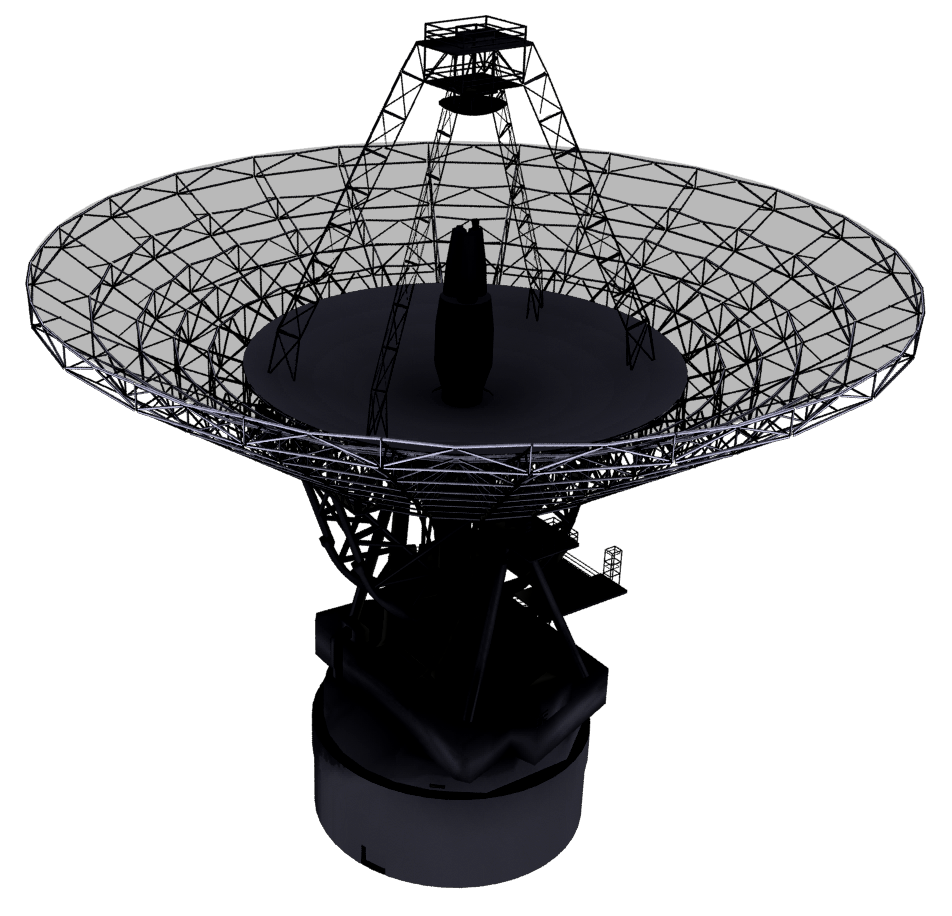
\includegraphics[height=0.85\paperheight]{fig/radar}%
    	};%
    	%\node[cog] (x) at (-1cm,3.6cm){};
    	%\node (d) [above of = x,node distance=1.4cm,label={[label distance=0.15cm,text=red]-20:$d(h,v)$}]{};
    	%\node (g) [below of = x,node distance=2.4cm,label={[label distance=0.15cm,text=red]20:$g$}]{};
    	%\path
	    %(x) edge [connect] (g)
	   	% 	edge [connect] (d);
	\end{tikzpicture}
\end{frame}


\section{Nonlinear-Gaussian state space models}

\begin{frame}
	\frametitle{Nonlinear-Gaussian SSMs}
	\vspace{-1cm}
	\note[itemize]{
		\item state
		\item static parameter
		\item dynamic model
		\item measurement model
		\item Markov chain
	}
	
	\begin{alignat*}{2}
		\xk &= \ff+\v{q}_{k-1}, \qquad& \v{q}_{k-1}&\sim \N{\v{0}}{\QQ}{\big} \\
		\yk &= \hh+\v{r}_{k}, & \v{r}_k&\sim \N{\v{0}}{\RR}{\big} \\
		\x_{0} &\sim \N{\muu}{\Sig}{\big}.
	\end{alignat*}
	
	\centering
	\begin{tikzpicture}
	\tikzstyle{main}=[circle, minimum size = 5mm, inner sep=0mm, thick, draw =black!80, node distance = 12mm,font=\small]
	\tikzstyle{param}=[circle, minimum size = 2mm, inner sep=0mm, thick, draw =white!80, fill=black!80, node distance = 18mm]
	\tikzstyle{ellipsis}=[circle, minimum size = 10mm, thick, draw =black!80, node distance = 18mm]
	\tikzstyle{connect}=[-latex, semithick]
	\tikzstyle{tconnect}=[-latex, thin, opacity=0.25]
	  \node[main] (x_1) [label=above:$\v{x}_{k-1}$] {};
	  \node[main,draw=black!0] (prev) [left of=x_1] {$\dots$};
	  \node[main] (x1) [left of=prev,label=above:$\v{x}_{0}$] {};
	  \node[main] (x) [right of=x_1,label=above:$\v{x}_{k}$] {};
	  \node[main] (x__1) [right of=x,label=above:$\v{x}_{k+1}$] {};
	  \node[main,fill = black!10] (y_1) [below of=x_1,label=below:$\v{y}_{k-1}$] {};
	  \node[main,fill = black!10] (y) [below of=x,label=below:$\v{y}_{k}$] {};
	  \node[main,fill = black!10] (y__1) [below of=x__1,label=below:$\v{y}_{k+1}$] {};
	  \node[main,fill = black!10] (y1) [below of=x1,label=below:$\v{y}_{0}$] {};
	  \node[main,draw=white!0] (next) [right of=x__1] {$\dots$};
	  \node[main] (xT) [right of=next,label=above:$\v{x}_{T}$] {};
	  \node[main,fill = black!10] (yT) [below of=xT,label=below:$\v{y}_{T}$] {};
	  \node[main,node distance=15mm] (theta) [above of=x,label=above:$\Th$] {};
	  \path
	    (x1) edge [connect] (prev)
	    	  edge [connect] (y1)
	    (prev) edge [connect] (x_1)
	    (x_1) edge [connect] (x) 
	    	  edge [connect] (y_1)
	    (x) edge [connect] (y)
	    	edge [connect] (x__1)
	    (x__1) edge [connect] (y__1)
	    	edge [connect] (next)
	    (next) edge [connect] (xT)
	    (xT) edge [connect] (yT)
	    (theta) edge [tconnect] (x__1)
	    	edge [tconnect] (x)
	    	edge [tconnect] (x_1)
	    	edge [tconnect] (x1)
	    	edge [tconnect] (xT)
	    	edge [tconnect] (y1)
	    	edge [tconnect] (y_1)
	    	edge [tconnect,bend left=20] (y)
	    	edge [tconnect] (y__1)
	    	edge [tconnect] (yT);
	\end{tikzpicture}
\end{frame}
	
\begin{frame}
	\frametitle{Static parameter estimation}
	\note{blaa}
\begin{itemize}
  \item Ultimate solution $\Pdf{\Th}{\Y}$ or $\Pdf{\X}{\Y}$
  \begin{itemize}
    \item particle filtering / sequential Monte Carlo
    \item too slow
  \end{itemize}
  \item Chosen strategy
  \begin{itemize}
    \item apply \emph{fast} Gaussian filtering and smoothing
    \item ML/MAP \emph{point} estimates 
    \end{itemize}
\end{itemize}

\end{frame}	


\section{Nonlinear gradient based optimization}

\begin{frame}
	\frametitle{Nonlinear gradient based optimization}
	\note{blaa}
	\begin{itemize}
	  \item log-LH $\lLH=\Pdf{\y_0}{\Th}+\sum_{k=1}^T \Pdf{\y_k}{\y_{0:k-1},\Th}$
	  \item Gaussian filter -> $\Pdf{\y_k}{\y_{1:k-1},\Th} \approx \N[\yk]{\v{\mu}_k}{\v{S}_k}$
	  \item score $\score[\Th']=\eval{\bm{\dpd{\lLH}{\theta_1} & \dots & \dpd{\lLH}{\theta_{d_\theta}}}^\tr}_{\Th=\Th'}$
	  \item sensitivity equations $\approx \dpd{\lLH}{\theta_i}$
	\end{itemize}
\end{frame}

\begin{frame}
	\frametitle{Quasi-Newton's methods}
	\note{blaa}
	\begin{itemize}
	  \item $\Th_{j+1} = \Th_j+\nabla^2\lLH[\Th_j]^{-1}\nabla\lLH[\Th_j]$
	  \begin{itemize}
	  	\item $\nabla^2\lLH[\Th_j]$ invertible?   
	  \end{itemize}
	  \item $\Th_{j+1} = \Th_j+\alpha_j\widehat{\v{H}}^{-1}_{j}\nabla\lLH[\Th_j]$
	  \begin{itemize}
	  	\item $\alpha_j$ is found by \emph{line search}
	  \end{itemize}
	  \item \emph{Broyden-Fletcher-Goldfarb-Shanno} (BFGS)
	  \begin{itemize}
	  	\item update rule for $\widehat{\v{H}}^{-1}_{j}$  
	  	\item only gradient needed
	  \end{itemize}
	  \item $\matlab$'s \texttt{fminunc}
	  \begin{itemize}
	  	\item BFGS
	  	\item cubic polynomial interpolation line search  
	  \end{itemize}
	\end{itemize}
\end{frame}

\section{EM}

\begin{frame}[plain]
\frametitle{Expectation Maximization (EM)}\vspace{-0.5cm}
\note{blaa}
$\lLH = \EMB{\v{\psi}}{\Th}+\KL{\tPX}{\post}$\\[0.4cm]
    \makebox[\textwidth]{
    	\centering
  		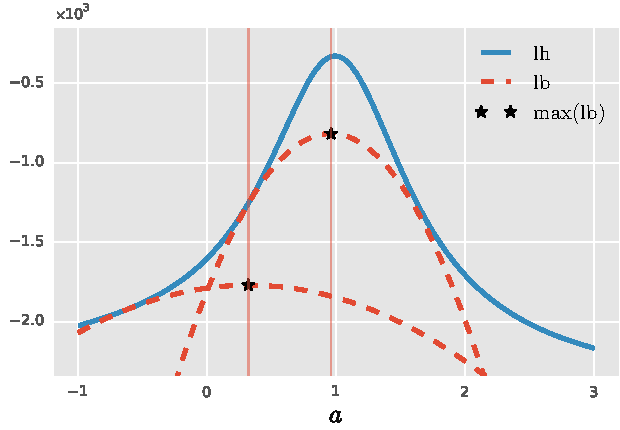
\includegraphics[width=0.9\textwidth]{../img/ar1_ex_em}
  	}
\end{frame}

\begin{frame}
	\frametitle{EM}
	\note{blaa}
\begin{description}
  \item[E-step]\hfill\\
  Set $\tPX{\v{\psi}_{j+1}}$ to the distribution that maximizes $\EMB{\v{\psi}}{\Th_j}$
  with respect to $\v{\psi}$. Here $\Th_j$ is the current estimate of $\Th$.  
  \item[M-step]\hfill\\ 
  Set $\Th_{j+1}$ to the estimate that maximizes $\EMB{\v{\psi}_{j+1}}{\Th}$ with respect to $\Th$.
\end{description}

In some sense, coordinate ascent in $\EMB{\v{\psi}}{\Th}$ 
\end{frame}



% \section{Fisher's identity}
% 
% \begin{frame}
% \frametitle{Score from EM}
% \[
% \score[\widehat\Th]=
% 		\nabla_{\Th}\EMQ[\big]{\widehat\Th}{\widehat\Th}
% 		\equiv\eval{\dpd{ \EMQ[\big]{\widehat\Th}{\Th}}{\Th}}_{\Th=\widehat\Th}
% \]
% \end{frame}

\section{Conclusion}
\begin{frame}
\frametitle{Conclusion}
\note{blaa}
	\begin{itemize}
		\item considered nonlinear SSMs
		\item MAP/ML estimates of static parameters
		\item gradient based nonlinear optimization of marginal log-likelihood
		\begin{itemize}
		    \item recursive sensitivity equations
		    \item possibly quadratic order of convergence
		\end{itemize}
		\item Expectation Maximization
		\begin{itemize}
		    \item linear-in-the-parameters -> no gradient computations
		    \item typically linear order of convergence
		\end{itemize}
		\item Fisher's identity
	\end{itemize}
\end{frame}
\begin{frame}
	\frametitle{Credits}
	\note{blaa}
	\begin{itemize}
	  \item Missile: Robert Kelly (dundaglan) \\ \url{http://www.blendswap.com}
	  \item DSN Dish: NASA \\ \url{http://www.nasa.gov/multimedia/3d_resources}
	\end{itemize}
\end{frame}




\end{document}